%!TEX root = ../../Master.tex
\subsection{Existing infrastructure in a hospital} \label{sub:infra}

\subsubsection{WiFi}

Most hospitals have good WiFi coverage around their cadastral. A visit to "Sygehus Nord" in Aalborg revealed that multiple locations around the hospital had a sufficient amount of WiFi hotspots in range, in order to use several of the positioning techniques covered in \cref{sub:pos}.

% \begin{figure}
% \centering
% 	\subcaptionbox{A cat\label{cat}}
% 	{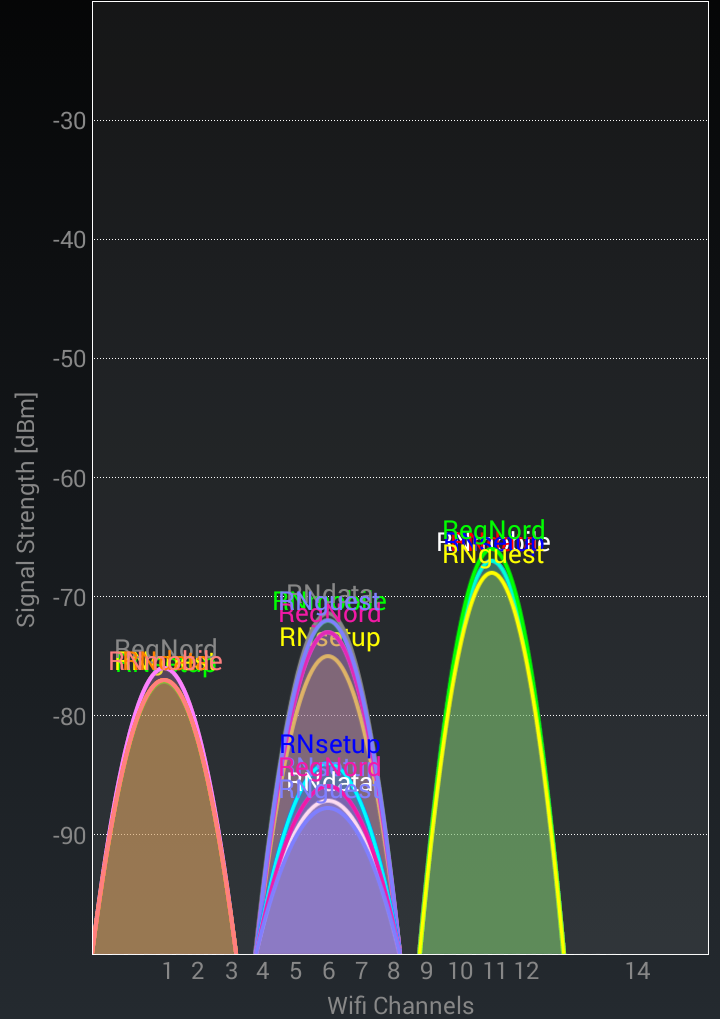
\includegraphics[width=\textwidth]{wifi_sygehus_nord1.png}}

% 		\subcaptionbox{A cat\label{cat}}
% 	{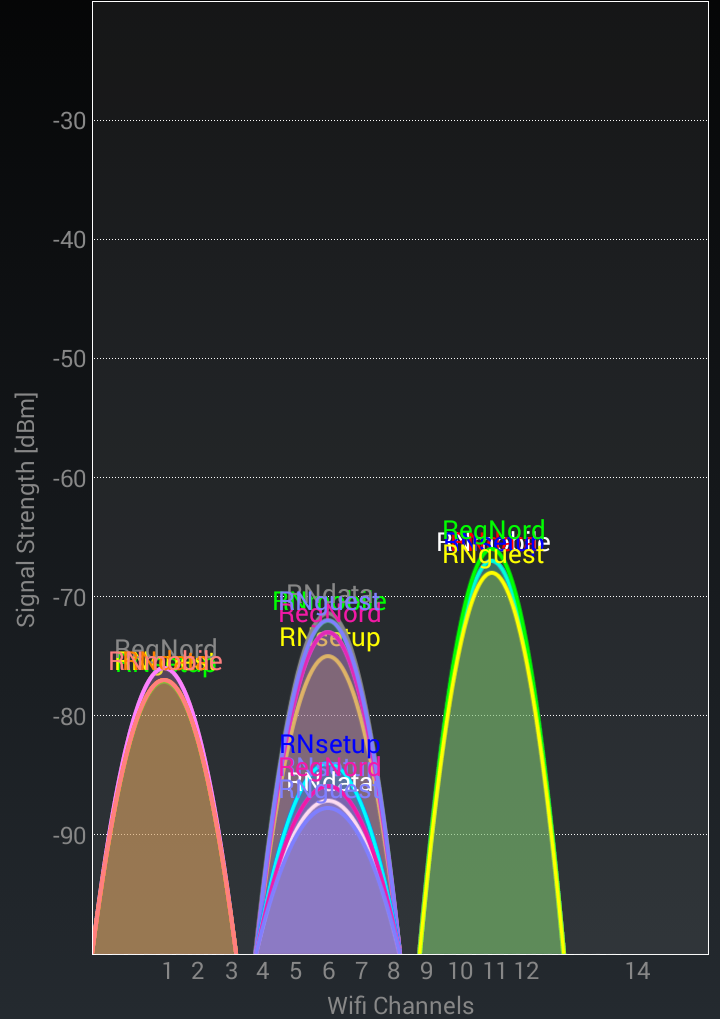
\includegraphics[width=\textwidth]{wifi_sygehus_nord1.png}}

% \end{figure}

\begin{figure}[htb]
	\begin{center} 
		\subcaptionbox{Graph of signal strength grouped by channels. Location A}
		{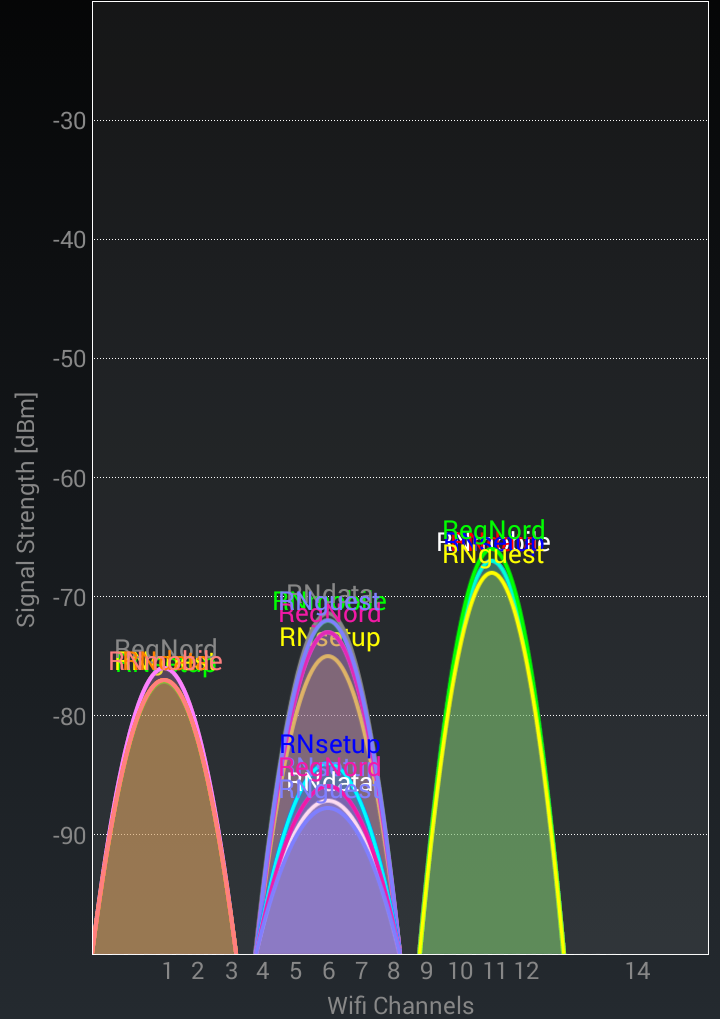
\includegraphics[width=0.33\textwidth]{wifi_sygehus_nord1.png}}
		\quad
		\subcaptionbox{Graph of signal strength grouped by channels. Location B}
		{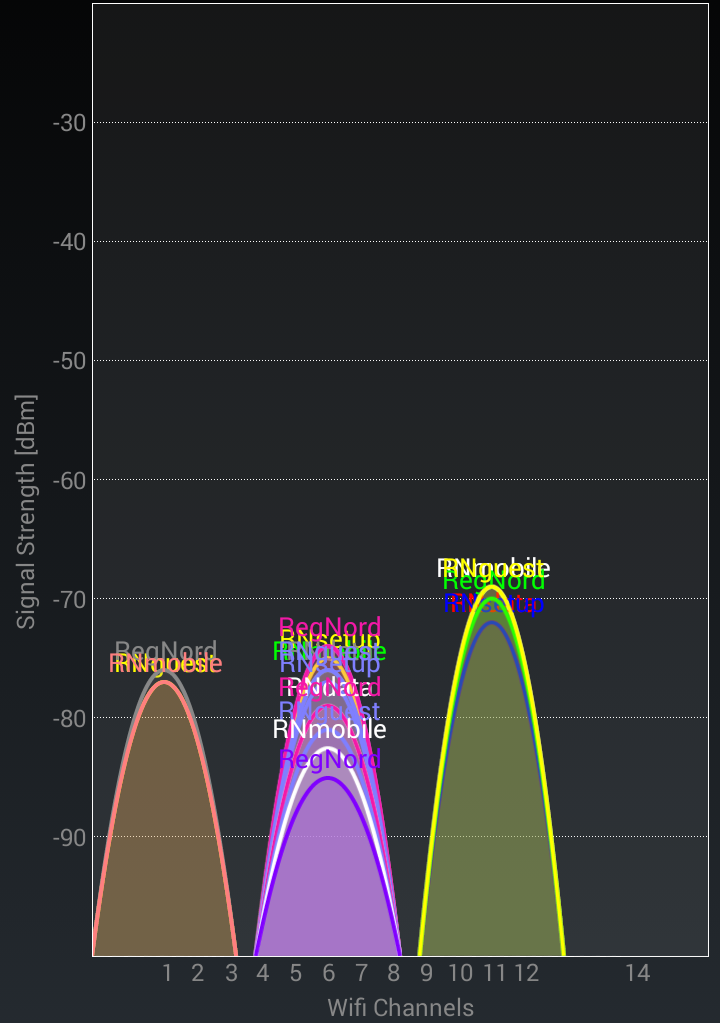
\includegraphics[width=0.33\textwidth]{wifi_sygehus_nord2.png}}
		\quad
		\subcaptionbox{List of WiFi networks}
		{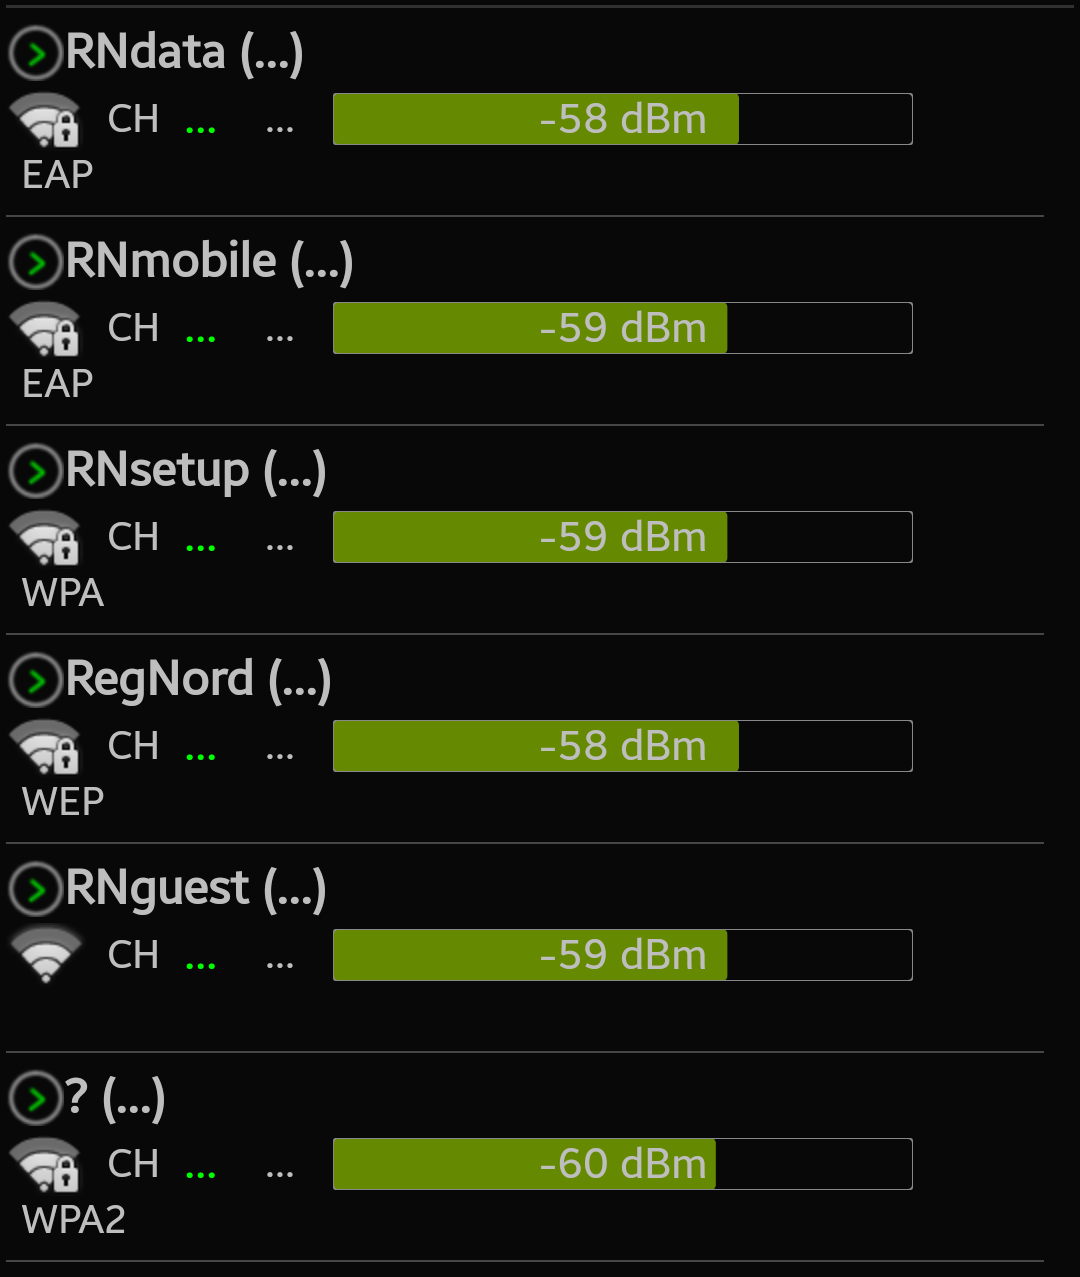
\includegraphics[width=0.33\textwidth]{wifi_sygehus_nord3.png}}
%\subfigure[label2][s]{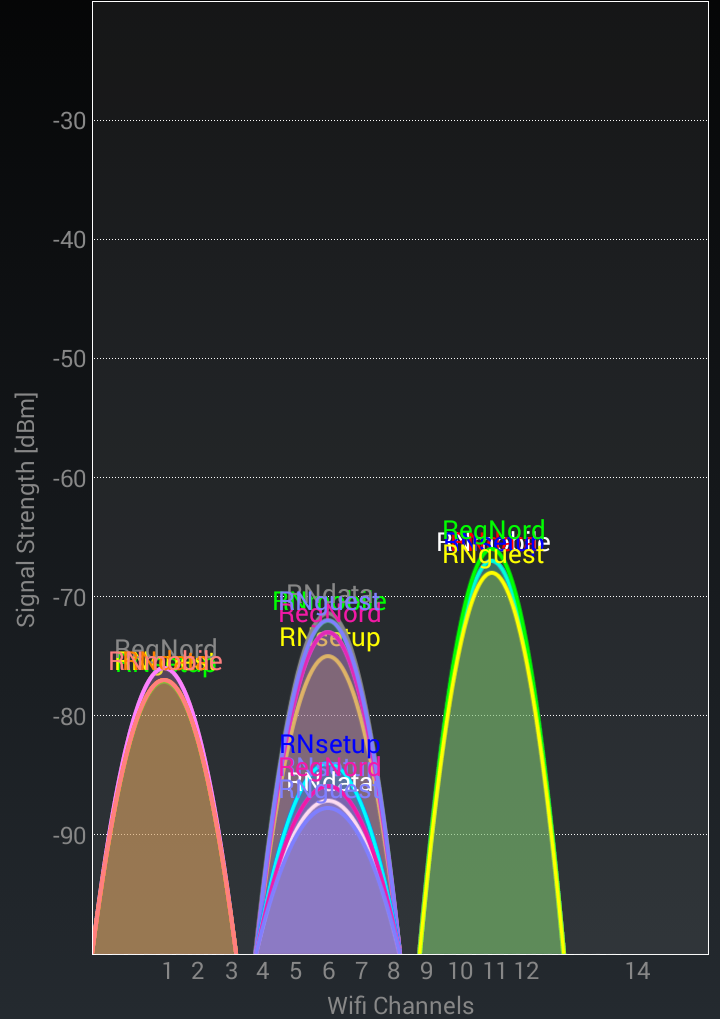
\includegraphics[]{wifi_sygehus_nord1.png}}
%\subfigure[label3][s]{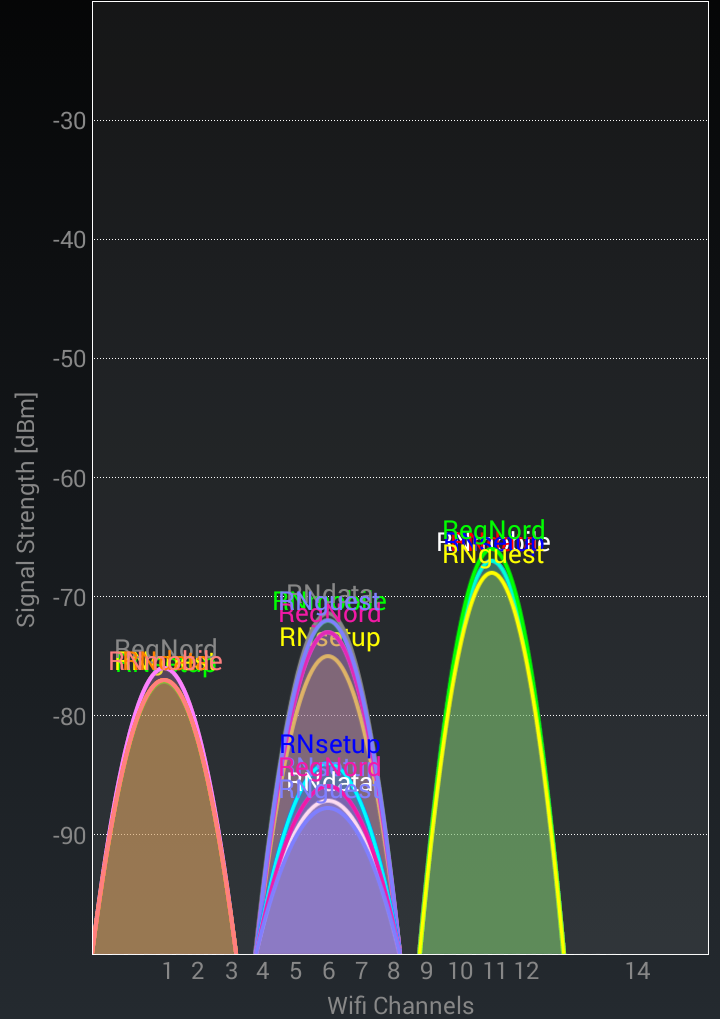
\includegraphics[]{wifi_sygehus_nord1.png}}
\end{center}
\caption{Analysis of wireless networks at Sygehus Nord Aalborg}
\label{fig:stefanResidual}
\end{figure}